\section{Introduction}

\subsection{Background}
\subsubsection[Overview]{History of Cryptocurrency}
\vspace*{-0.5cm}

\begin{minipage}[h]{0.45\linewidth}
%Print version of table
\begin{warpprint}
\begin{table}[H]{}
\renewcommand\arraystretch{1.4}\arrayrulecolor{blue}
\captionsetup{singlelinecheck=false, labelfont=sc, labelsep=quad}
\caption{Timeline of Cryptocurrency}%\vskip -1.5ex
% lwarp table, and print edition (uncomment stuff below for good copy)
\begin{tabular}{c p{5cm}}%
% Good copy for print edition
%\begin{tabular}{@{\,}r <{\hskip 2pt} !{\foo} >{\raggedright\arraybackslash}p{5cm}}
%\toprule
%\addlinespace[1.5ex]
2008 & Bitcoin White Paper \\
2009 & Bitcoin Genesis Block\\
2013 & 1 BTC = \$ 31 USD\\
2013 & \gls{Ethereum} White Paper \\
2015 & \gls{Ethereum} Genesis Block\\
2015 & \gls{HyperLedger} starts \\
2017 & Over 1000 different cryptocurrencies \\
2018 & AWS Blockchain Templates \\
\end{tabular}
\end{table}
\end{warpprint}
% HTML VERSION OF TABLE
\begin{warpHTML}
\begin{table}[H]{}
\renewcommand\arraystretch{1.4}\arrayrulecolor{blue}
%\captionsetup{singlelinecheck=false, labelfont=sc, labelsep=quad}
\caption{Timeline of Cryptocurrency}%\vskip -1.5ex
% lwarp table, and print edition (uncomment stuff below for good copy)
\begin{tabular}{c p{5cm}}%
% Good copy for print edition
%\begin{tabular}{@{\,}r <{\hskip 2pt} !{\foo} >{\raggedright\arraybackslash}p{5cm}}
%\toprule
%\addlinespace[1.5ex]
2008 & Bitcoin White Paper \\
2009 & Bitcoin Genesis Block\\
2013 & 1 BTC = \$ 31 USD\\
2013 & \gls{Ethereum} White Paper \\
2015 & \gls{Ethereum} Genesis Block\\
2015 & \gls{HyperLedger} starts \\
2017 & Over 1000 different cryptocurrencies \\
2018 & AWS Blockchain Templates \\
\end{tabular}
\end{table}
\end{warpHTML}
\end{minipage}%
\begin{minipage}[h]{0.55\linewidth}
In 2008 bitcoin white paper \cite{bitcoinWhitePaper:Online} described a way to solve the double spending problem without a centralized body using \gls{blockchain}. Although, the value of bitcoin (BTC) has grown exponentially, high computational and energy consumption in mining and slow performance \cite{bitCoinProblems:Online}.  Released in July 30, 2015, Ethereum, an open-source platform based on blockchain technology, distinguishes itself from bitcoin through faster transactions, unlimited processing capability for \glspl{smart contract}, and its network is optimized to support \gls{DApp} \cite{ethereumWhitePaper:Online}.
\end{minipage}%
%\begin{figure}[ht]
%\begin{adjustbox}{center,max width=1.1\textwidth}
%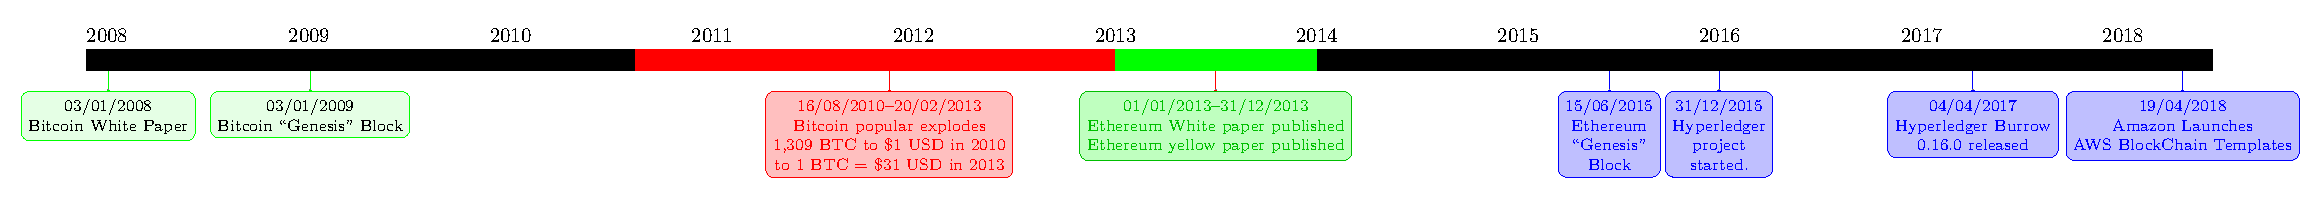
\includegraphics[width=1.2\linewidth]{Diagrams/advancedTimeline.pdf}
%\end{adjustbox}
%\caption{An example of server-blockchain architecture in a DAPP.}
%\label{fig:dappArc}
%\end{figure}



%%% Contain timeline
\vspace*{-0.25cm}
\subsubsection{Decentralized Applications}
%%% ClEAN TIHS UP LATER
	%A blockchain is a digitized, decentralized, public ledger of all cryptocurrency transactions. %To access websites on the Ethereum blockchain and use dapps a specialized browser is needed, or a browser plugin like \gls{MetaMask}. 
	Blockchain technology is revolutionizing the internet by establishing trust in shared data. \cite{book:bchainForDummies}.
	Additionally, transactions recorded on the blockchain are practically impossible to remove or change. 
	
	
	\begin{warpprint}
	\begin{figure}[ht]
	%\begin{adjustbox}{center,max width=1.1\textwidth}
	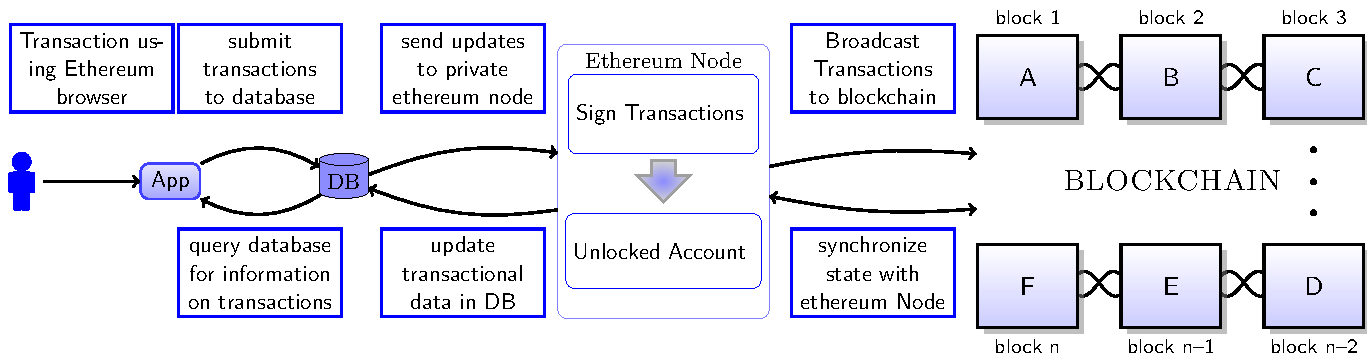
\includegraphics[width=1\linewidth]{Diagrams/blockchainInSimpleApp.pdf}
	%\end{adjustbox}
	\caption{An example of server-blockchain architecture in a DAPP.}
	\label{fig:DApp}
	\end{figure}
	\end{warpprint}
	
	\begin{warpHTML}
	\begin{figure}[ht]
	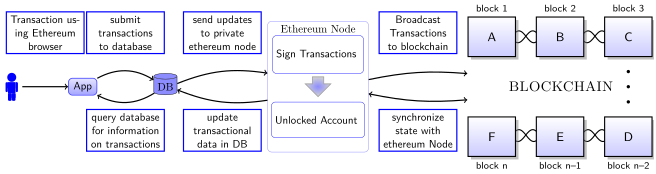
\includegraphics[width=1.2\linewidth]{Diagrams/blockchainInSimpleApp.svg}
	\caption{An example of server-blockchain architecture in a DAPP.}
	\label{fig:DApp}
	\end{figure}
	\end{warpHTML}
	
	A decentralized application, or DApp are deployed on peer to peer networks such as Ethereum or on the cloud \footnotemark. A decentralized system (peer to peer) has many advantages over a conventional centralized network including no single points of failure, cheaper distribution (servers are expensive), faster upload speeds. 
	\footnotetext[1]{Amazon recently started offering blockchain templates on AWS. %\cite{ethereumWhitePaper:Online}
	}
	
	%\paragraph{Types of Blockchains}
	%\begin{itemize}
	%\item[---]  \textbf{Public blockchains} are large distributed networks that are run through a native token such as bitcoin or ether. Anyone can participate and the community maintains its open-source code. The two largest public blockchains are Ethereum and Bitcoin.%They’re open for anyone to participate at any level and have open-source code that their community maintains.
	% rewrite and add section about composer
	%\item[---] \textbf{Permissioned blockchains} define role based access control for individuals in the network and uses native tokens.  \gls{HyperLedger Composer}, an open-source framework for permissioned blockchains, is used for smart contracts and for blockchain application development \cite{hyperledgerComposer:Online}. One use case is an accounting system that calculates payment, while hiding that information from unrelated organizations.  % Their core code may or may not be open source.
	%\item[---] \textbf{Private blockchains}  membership is tightly controlled and lacks a native token. Useful for consortiums with trusted associates and exchanging confidential information, however, less powerful because it is supported by limited private resources.
	%\end{itemize}
	%\vspace*{-0.5cm}
	
	
	% Consider taking this part out, too detailed for the high level explaination.
	\paragraph{Public and Private Keys}
	 \textbf{In a blockchain} system, any key holder can use their private key to sign a piece of data. This results in a signature.  
	  In a Dapp, this can be used for:
	 \begin{enumerate}
		\item Recovering the public key (ethereum account address) of the Author.
		\item Verify if the raw data is identical  using the Author's public key. 
	\end{enumerate}
	
	%In order to sign something, a mathematical function is used to "sign" a piece of document/data. A digital signature of a document/data is a number generated using a private key. The private key has a corresponding public key. 
	
	
	
%	\begin{figure}[ht]
%	\centering
%	
\includegraphics[width=0.5\linewidth]{Diagrams/verifySig.png}
%	\caption{Illustrate how public and private keys are used to verify signatures}
%	\label{fig:verfSig}
%	\end{figure}
	
		 
% refer to medium article, and some other article highlighting the interest in private nodes, https://aws.amazon.com/partners/blockchain/
% https://blog.zeppelin.solutions/designing-the-architecture-for-your-ethereum-application-9cec086f8317
% https://aws.amazon.com/blogs/apn/introducing-aws-blockchain-partners/

%		To access websites on the Ethereum blockchain and use dapps a specialized browser is needed, or a plugin like metamask. 

\subsubsection{Smart Contracts}
%	\begin{minipage}[h]{0.5\linewidth}
		Traditional legal contracts are written to represent the contracting parties. In a smart contract, self-executing source code is used to automatic transactions that are publicly available on the blockchain \cite{ethereumWhitePaper:Online}.
		Furthermore, smart contracts allow buyers and sellers exchange money, property, shares, or anything of value in a transparent, conflict-free way while avoiding the services of a middleman. This allows validation of complex transactions swiftly while maintaining transparency. Although the benefits of using smart contracts are obvious, legal enforceability is difficult because "no central administering authority to decide a dispute" exists \cite{keyfindings:Online}. 
		
		In addition, irreversible and immutable transactions are a disadvantage that hackers can exploit. For example, an amateur coder killed the contract that allowed users to transfer Ether for the Parity Ethereum Wallet, rendering 150 to 300 million dollars completely useless \cite{funnyJoke:Online}. Scrutinizing smart contracts and reducing bugs in production code is essential. An example of smart contract is available in Appendix A \ref{lst:label}.
%	\end{minipage}
%	\begin{minipage}[h]{0.5\linewidth}
%		\begin{lstlisting}[language=Solidity,caption=Smart contract in Solidity]
%		// pragma is used to specifc version of Solidity
%		pragma solidity ^0.4.16;
%		contract HelloWorld {
%		 uint256 counter = 5; 
%		 //state variable we assigned earlier
%		 address owner = msg.sender; 
%		 //set owner as msg.sender
%		function add() public {  //increases counter by 1
%	  		counter++;
%		 }
%		 function subtract() public { //decreases counter by 1
%		  counter--;
%		 }
%		 function getCounter() public constant returns (uint256) {
%		  return counter;
%		 } 
%		 function kill() public { //self-destruct function, 
%		   if(msg.sender == owner) {
%		    selfdestruct(owner); 
%		   }
%		}
%		
%		// Fallback function
%		function () public payable {
%		
%		 }
%		\end{lstlisting}
%	\end{minipage}

	\begin{warpprint}
	\begin{figure}[ht]
		\centering
		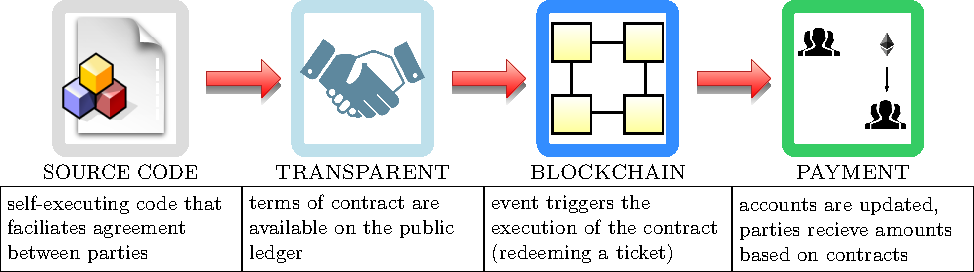
\includegraphics[width=1\linewidth]{Diagrams/smartContractsExp.pdf}
		\caption{Illustrating how a smart contract works}
		\label{fig:smartContracts}
	\end{figure}
	\end{warpprint}
	
	\begin{warpHTML}
	\begin{figure}[ht]
		\centering
		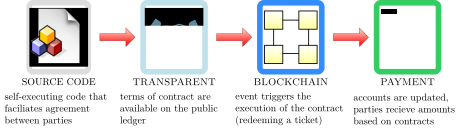
\includegraphics[width=1\linewidth]{Diagrams/smartContractsExp.svg}
		\caption{Illustrating how a smart contract works}
		\label{fig:smartContracts}
	\end{figure}
	\end{warpHTML}
%	\newpage
	
	
%	or internal processes such as supply chains, a private blockchain makes sense (data cannot be changed) and cryptographic auditing with known identities (public keys). For a trustless system, using a public blockchain makes the most sense. In comparsion, a permissioned blockchain is effective for limiting what can or cannot do, as well as prevent users from seeing other transactions they are not suppose to see.
	
	%Despite the slow speed of the public blockchain, innovations such as \gls{side chains} enable quick transactions and are used in blockchain game development \cite{loomNetwork:Online}. % 
	

\subsection{Objective}
The prominence of cryptocurrency and decentralized applications suggests usage of smart contracts will experience explosive growth.

\subsubsection{Problem}

Currently commonplace transactions require days to process and for parties verify correctness. For example to purchase houses, a plethora of steps are required, one must interactive with lawyers, real-estate agents, home inspector, buy insurance and shop for a mortgage. 

\subsubsection{Purpose}
Leveraging existing blockchain technologies can automatic the majority of steps and cut out the middlemen, resulting in buyers conversing directing with sellers.
% Although smart contracts have immense potential to simplify transactions, issues such as limiting access to information, latency when updating (takes 10 minutes to write info to bitcoin blockchain), and immutability of translations (cannot undo transfer of assets) must be addressed.
% See https://www.cs.auckland.ac.nz/research/groups/ssg/homepages/yu-cheng/ytu001_PhDThesis.pdf
% https://researchspace.auckland.ac.nz/handle/2292/22092
\subsection{Aims}
The aims of this project are to develop a decentralized blockchain system that:
\begin{enumerate}
\item Reduce cost of transactions by at least 50\% from removing middlemen.
\item Improve transparency in software systems through augmented accessibility and understandability.
\item Increased security and greater enforceability of contractual obligations.
%1. Uses 15% less material to decrease cost and weight.
%2. Has improved efficiency by reducing the air gap by 10%.
%3. Has no reduction in its reliability or increase in its maintenance requirements. 
\end{enumerate}
\subsubsection{Limitations}

The regulatory uncertainty and impact of future regulations on blockchain technologies such as smart contracts will not be investigated. In addition, criminal usage of cryptocurrencies to avoid taxation and legal repercussions are beyond the scope of this report. In addition the impacts of quantum computing altering the validity of modern cryptography algorithms will not be investigated.
%The performance of the linear generator in extreme storm events will not be investigated as this
%cannot be accurately modeled using Airy linear wave theory. This project will be based on
%numerical simulations; no physical model will be tested to validate the results.

\newpage  
